\documentclass[14pt]{beamer}

\definecolor{todocolor}{rgb}{1, 0.3, 0.2}
\newcommand{\td}[1]{\colorbox{todocolor}{*\footnote{TODO: #1}}}


% normally included with amsart
% \usepackage{amsmath, amsthm}

% font with unicode support, does not work with classicthesis
% \usepackage{fontspec}

% clickable tocs
\usepackage{hyperref}

% floating figures
\usepackage{float}

% for multiple cites
\usepackage{cite}

% fancy diagrams
% \usepackage{tikz}
% \usetikzlibrary{matrix, arrows, decorations}
% \tikzset{node distance=2.5em, row sep=2.2em, column sep=2.7em, auto}

% simple diagrams
\usepackage[all,cmtip]{xy}

\usepackage{graphicx}
\graphicspath{ {./images/} }
\usepackage{caption}
\usepackage{subcaption}

% for the fib arrow
\usepackage{amssymb}

% Some basic objects
\newcommand{\N}{\mathbb{N}}				% natural numbers
\newcommand{\Np}{{\mathbb{N}^{>0}}}		% positive numbers
\newcommand{\Z}{\mathbb{Z}}				% integers
\newcommand{\R}{\mathbb{R}}				% reals
\DeclareRobustCommand{\Q}{\mathbb{Q}}				% rationals
\renewcommand{\k}{\mathrm{I\!k}}		% default ground ring

% Basic category stuff
\newcommand{\cat}[1]{\mathbf{#1}}		% the category of ...
\newcommand{\opCat}[1]{{#1}^{\text{op}}}% opposite category
\newcommand{\Hom}{\mathbf{Hom}}
\newcommand{\id}{\mathbf{id}}
\newcommand{\Ho}{\cat{Ho}}

% Categories
\newcommand{\Set}{\cat{Set}}			% sets
\newcommand{\Top}{\cat{Top}}			% topological spaces
\newcommand{\Grp}{\cat{Grp}}			% groups
\newcommand{\Ab}{\cat{Ab}}				% abelian groups
\newcommand{\DELTA}{\boldsymbol{\Delta}}% the simplicial cat
\newcommand{\simplicial}[1]{\cat{s{#1}}}% simplicial objects
\newcommand{\sSet}{\simplicial{\Set}}	% simplicial sets
\newcommand{\Mod}[1]{\cat{{#1}Mod}}		% modules over a ring
\newcommand{\Alg}[1]{\cat{{#1}Alg}}		% algebras over a ring
\newcommand{\grMod}[1]{\cat{gr\mbox{-}{#1}Mod}}	% graded modules over a ring
\newcommand{\grAlg}[1]{\cat{gr\mbox{-}{#1}Alg}}	% graded algebras over a ring
\newcommand{\dgMod}[1]{\cat{dg\mbox{-}{#1}Mod}}	% differential graded modules over a ring
\newcommand{\dgAlg}[1]{\cat{dg\mbox{-}{#1}Alg}}	% differential graded algebras over a ring
\newcommand{\Ch}[1]{\cat{Ch_{n\geq0}({#1})}}	% chain complexes
\newcommand{\CoCh}[1]{\cat{Ch^{n\geq0}({#1})}}	% cochain complexes
\DeclareRobustCommand{\DGA}{\cat{DGA}}			% cochain algebras
\DeclareRobustCommand{\CDGA}{\cat{CDGA}}		% commutative cochain algebras
\DeclareRobustCommand{\AugCDGA}{\cat{CDGA^\ast}}% augmentedcommutative cochain algebras

\newcommand{\cof}{\hookrightarrow}		% cofibration
\newcommand{\fib}{\twoheadrightarrow}	% fibration
\newcommand{\we}{\tot{\simeq}}			% weak equivalence

% for use in xy diagrams
\newcommand{\arcof}{\ar@{^{(}->}}
\newcommand{\artcof}{\ar@{^{(}->}|\simeq}
\newcommand{\arfib}{\ar@{->>}}
\newcommand{\artfib}{\ar@{->>}|\simeq}
\newcommand{\arwe}{\ar|-\simeq}
\newcommand{\ariso}{\ar|-\iso}

% adjunction symbol for xymatrices
\newcommand{\xyadj}{\raisebox{0.2\height}{\scalebox{0.5}{$\perp$}}}

% pushout and pullback for xymatrices (makes empty arrow with text)
\newcommand{\xypo}{\ar@{}[dr]|(.75){\scalebox{1.2}{$\ulcorner$}}}
\newcommand{\xypb}{\ar@{}[dr]|(.25){\scalebox{1.2}{$\lrcorner$}}}

%\newcommand{\leftadj}{\ooalign{\hss\rightleftarrows\hss\cr\bot}}
\newcommand{\leftadj}{\rightleftarrows}

% Notation and operators
\newcommand{\I}{\,\mid\,}				% seperator in set notation
\newcommand{\del}{\partial}				% boundary
\newcommand{\iso}{\cong}				% isomorphic
\newcommand{\eq}{\sim}					% homotopic
\newcommand{\ison}[1]{\stackrel{(#1)}{\iso}} % isos to refer to
\newcommand{\refison}[1]{{\small $(#1)$}}    % ref
\newcommand{\tot}[1]{\xrightarrow{\,\,{#1}\,\,}}	% arrow with name
\newcommand{\toti}[1]{\xleftarrow{\,\,{#1}\,\,}}	% left arrow with name
\newcommand{\mapstot}[1]{\xmapsto{\,\,{#1}\,\,}}	% mapsto with name
\newcommand{\unit}{\eta}
\newcommand{\counit}{\epsilon}
\DeclareMathOperator*{\im}{im}
\DeclareMathOperator*{\coker}{coker}
\DeclareMathOperator*{\colim}{colim}
\DeclareMathOperator*{\Tor}{Tor}
\DeclareMathOperator*{\Ext}{Ext}
\DeclareMathOperator*{\tensor}{\otimes}
\DeclareMathOperator*{\bigtensor}{\bigotimes}
\renewcommand{\deg}[1]{{|{#1}|}}
\newcommand{\Char}[1]{char({#1})}
\newcommand{\RH}{\widetilde{H}}			% reduced homology
\DeclareRobustCommand{\C}{\mathcal{C}}			% Serre mod C class
\newcommand{\Apl}[0]{{A_{PL}}}			% Apl simplicial set of polynomials

\newcommand{\titleCDGA}{\texorpdfstring{$\CDGA$}{CDGA}}

% restriction of a function
\newcommand\restr[2]{{% we make the whole thing an ordinary symbol
  \left.\kern-\nulldelimiterspace % automatically resize the bar with \right
  #1 % the function
  \vphantom{\big|} % pretend it's a little taller at normal size
  \right|_{#2} % this is the delimiter
  }}


\theoremstyle{plain}
\newtheorem{theorem}{Theorem}[section]
\newtheorem{proposition}[theorem]{Proposition}
\newtheorem{lemma}[theorem]{Lemma}
\newtheorem{corollary}[theorem]{Corollary}
\newtheorem{claim}[theorem]{Claim}
\newtheorem{remark}[theorem]{Remark}

\theoremstyle{definition}
\newtheorem{definition}[theorem]{Definition}
\newtheorem{notation}[theorem]{Notation}
\newtheorem{example}[theorem]{Example}

\newcommand{\EnvTemp}[4]{
	\begin{#1}\label{#2:#3}
		{#4}
	\end{#1}
}

\newcommand{\RefTemp}[3]{{#1}~\ref{#2:#3}}

\newcommand{\Theorem}{\EnvTemp{theorem}{thm}}
\newcommand{\Proposition}{\EnvTemp{proposition}{prop}}
\newcommand{\Lemma}{\EnvTemp{lemma}{lem}}
\newcommand{\Corollary}{\EnvTemp{corollary}{cor}}
\newcommand{\Claim}{\EnvTemp{claim}{clm}}
\newcommand{\Remark}{\EnvTemp{remark}{rmk}}
\newcommand{\Proof}[1]{\begin{proof}{#1}\end{proof}}

\newcommand{\Def}{\emph}
\newcommand{\Definition}{\EnvTemp{definition}{def}}
\newcommand{\Notation}{\EnvTemp{notation}{not}}
\newcommand{\Example}{\EnvTemp{example}{eg}}

\newcommand{\TheoremRef}{\RefTemp{Theorem}{thm}}
\newcommand{\LemmaRef}{\RefTemp{Lemma}{lem}}
\newcommand{\CorollaryRef}{\RefTemp{Corollary}{cor}}
\newcommand{\RemarkRef}{\RefTemp{Remark}{rmk}}

\newcommand{\DefinitionRef}{\RefTemp{Definition}{def}}

\newcommand{\Chapter}[2]{\chapter{#1}\label{chp:#2}}
\newcommand{\ChapterRef}{\RefTemp{Chapter}{chp}}

% headings for a table
\newcommand*{\thead}[1]{\multicolumn{1}{c}{\bfseries #1}}

% simple way to center an image
\newcommand{\cimage}[2][]{
	\begin{center}
	\includegraphics[#1]{#2}
	\end{center}
}

% simple way to center a diagram
\newcommand{\cdiagrambase}[1]{
	\begin{displaymath}
	\input{#1}
	\end{displaymath}
}
\newcommand{\cdiagram}[1]{
	\cdiagrambase{diagrams/#1}
}

\usepackage{tabularx}
\renewcommand{\tabularxcolumn}[1]{p{#1}}

\graphicspath{ {../presentation/images/} }

\newcommand{\Frame}[2]{
	\begin{frame}{#1}#2\end{frame}
}

\title{Rational Homotopy Theory}
\author{Joshua Moerman}
\institute[Radboud Universiteit Nijmegen]{Supervisor: Ieke Moerdijk}
\date{}

\begin{document}

\AtBeginSection[]{
	\begin{frame}<beamer>
		\tableofcontents[currentsection]
	\end{frame}
}

\Frame{}{
	\titlepage
}


\section{Introduction to homotopy theory}
\Frame{Homotopy theory}{
	\begin{center}
	Study of spaces or shapes \\
	with ``weak equivalences''

	\bigskip
	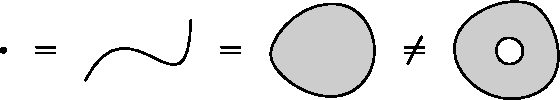
\includegraphics{weak_eqs2}
	\end{center}
}

\Frame{Important spaces}{
\begin{align*}
	S^1 &= \raisebox{-0.4\height}{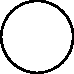
\includegraphics{spheres1}} \\[1em]
	S^2 &= \raisebox{-0.4\height}{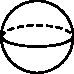
\includegraphics{spheres2}} \\[1em]
	S^3 &= \>\> \cdots \\[1em]
	    &\>\> \vdots
\end{align*}
}

\Frame{Important tool}{
	Fundamental group:

	\[ \pi_1(X) = \text{maps } S^1 \to X \text{ up to homotopy} \]

	\bigskip
	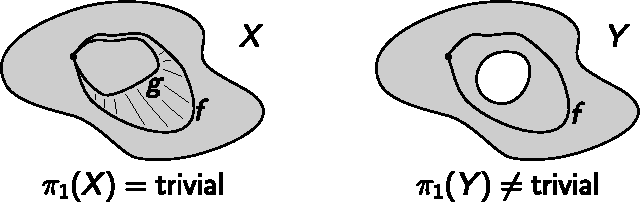
\includegraphics{fundamental_group}
}

\Frame{Important tools}{
	Homotopy groups:

	\begin{align*}
	\pi_1(X) &= \text{maps } S^1 \to X \text{ up to homotopy} \\[1em]
	\pi_2(X) &= \text{maps } S^2 \to X \text{ up to homotopy} \\[1em]
	\pi_3(X) &= \text{maps } S^3 \to X \text{ up to homotopy} \\[1em]
	&\>\>\vdots
	\end{align*}
}

\Frame{Torsion-free}{
	Serre proved in 1950s:
	\begin{align*}
		\text{odd } k: \quad \pi_n(S^k) \tensor \Q &=
		\begin{cases}
			\Q &\text{ if } n = k \\
			0 &\text{ otherwise }
		\end{cases} \\[1em]
		\text{even } k: \quad \pi_n(S^k) \tensor \Q &=
		\begin{cases}
			\Q &\text{ if } n = k, 2k-1 \\
			0 &\text{ otherwise }
		\end{cases} \\
	\end{align*}
}


\section{Rational homotopy theory}
\Frame{Rational homotopy theory}{
	\begin{center}
	Study of spaces\\
	with ``rational equivalences'' \\
	and ``rational homotopy groups''

	\pause
	\bigskip
	or
	\bigskip

	Study of \emph{rational} spaces \\
	with weak equivalences \\
	and ordinary homotopy groups
	\end{center}
}

\Frame{Rational spaces}{
	$X$ is \emph{rational} if $\pi_n(X)$ is a $\Q$-vector space

	\bigskip
	\[ S^1_\Q = \raisebox{-0.55\height}{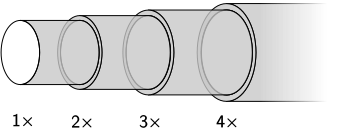
\includegraphics{infinite_telescope}} \]
}


\section{The main equivalence}
\Frame{Main equivalence}{
	\begin{theorem}
	\begin{center}
		Homotopy theory of rational spaces \\
		= \\
		Homotopy theory of commutative differential graded algebras
	\end{center}
	\end{theorem}
}

\Frame{Main equivalence (precise version)}{
	\begin{theorem}
		\[ \Ho(\Top_{\Q, 1, f}) \simeq \opCat{\Ho(\CDGA_{\Q, 1, f})} \]
	\end{theorem}
}

\Frame{What is a cdga?}{
	\begin{definition}
		a cdga $A$ is
		\begin{itemize}
			\item a $\Q$-vector space
			\item with a multiplication $A \tensor A \tot{\mu} A$
			\item with a differential $A \tot{d} A$ such that $d^2 = 0$
			\item with a grading $A = \bigoplus_{n \in \N} A^n$
			\item it is commutative: $ x y = (-1)^{\deg{x}\cdot\deg{y}} y x $
		\end{itemize}
	\end{definition}
}

\Frame{Free cdga's}{
	As always: there is a free guy: $\Lambda(...)$

	For example
	\[ \Lambda(t, dt) \text{ with } \deg{t} = 0 \]
	is just polynomials in $t$, with its differential $dt$
}

\newcommand{\Dict}[1]{
	\noindent
	\begin{tabularx}{\textwidth}{ X X }
		{\bf rational spaces} & {\bf cdga's} \\[1em]
		#1
	\end{tabularx}
}

\Frame{Dictionary}{
	\Dict{
		$S^n_\Q$ with $n$ odd
				& $\Lambda(e)$ with $\deg{e} = n$ \\[1em]

		$S^n_\Q$ with $n$ even
				& $\Lambda(e, f)$ with $\deg{e} = n$, $\deg{f} = 2n-1$ and $d f = e^2$ \\[1em]

		Eilenberg-MacLane space $K(\Q, n)$
				& $\Lambda(e)$ with $\deg{e} = n$
	}
}

\Frame{Dictionary}{
	\Dict{
		weak equivalence $$\pi_n(f): \pi_n(X) \iso \pi_n(Y)$$
				& weak equivalence $$H(f): H(X) \iso H(Y)$$ \\[1em]

		homotopy $$h: X \times I \to Y$$
				& homotopy $$h: A \to B \tensor \Lambda(t, dt)$$
	}
}

\Frame{Dictionary}{
	\Dict{
		$$ \pi_n(X) = [S^n, X] $$
				& {\begin{align*}
					\pi^n(A) &= H(Q(A)) \\
					\pi^n(A)^\ast &\iso [A, \Lambda(e)] \\
					              &\text{or } [A, \Lambda(e, f)]
				\end{align*}} \\[1em]

		Long exact sequence of a fibration
				& Long exact sequence of a cofibration \\[1em]
	}
}

\Frame{Dictionary}{
	\bf topological $n$-simplex
	\[ \Delta^n = \left\{ (x_0, \ldots, x_n) \in \R^{n+1} \,|\, \sum x_i = 1, x_i \geq 0 \right\} \]

	\bigskip
	\bf cdga $n$-simplex
	\[ \Delta_n = \frac{\Lambda(x_0, \ldots x_n, dx_0, \ldots, dx_n)}{\langle \sum x_i - 1, \sum dx_i \rangle} \]
}

\Frame{Construction}{
	\begin{center}
	\begin{tikzcd}[column sep=huge, row sep=huge, ampersand replacement=\&]
		\DELTA \arrow[d, "y"] \arrow[rd, "\Delta_{(-)}"] \& \\
		\sSet \arrow[r, dashed, shift left = 1ex, "A"] \& \opCat{\CDGA_\Q} \arrow[l, dashed, shift left = 1ex]
	\end{tikzcd}
	\end{center}

	\bigskip
	\pause
	\[ A(X) = \Hom_\sSet(X, \Delta_{(-)}) \]
}


\end{document}
